% Copyright(C) 2011-2015 Pedro H. Penna <pedrohenriquepenna@gmail.com>
%
% This file is part of Nanvix.
%
% Nanvix is free software; you can redistribute it and/or modify
% it under the terms of the GNU General Public License as published by
% the Free Software Foundation; either version 3 of the License, or
% (at your option) any later version.
%
% Nanvix is distributed in the hope that it will be useful,
% but WITHOUT ANY WARRANTY; without even the implied warranty of
% MERCHANTABILITY or FITNESS FOR A PARTICULAR PURPOSE. See the
% GNU General Public License for more details.
%
% You should have received a copy of the GNU General Public License
% along with Nanvix. If not, see <http://www.gnu.org/licenses/>.

\documentclass[10pt,a4paper]{article}

% Input.
\usepackage[utf8]{inputenc}
\usepackage[english]{babel}

% Figures.
\usepackage{graphicx}

% References.
\usepackage[backend=biber]{biblatex}

\author{Pedro H. Penna}
\title{The Nanvix Operating System}

\begin{document}

\maketitle

\section{Introduction}
\label{section: introduction}

% About Nanvix.
Nanvix is an operating system created by Pedro H. Penna for educational purposes. It was designed from scratch to be small and simple, and yet modern and fully featured, so that it could help both, novices and experienced enthusiasts in operating systems, to learn about kernel hacking. The first release of Nanvix came out in early 2011, and since then the system has gone through several changes. This paper details the internals of Nanvix 1.2. All previous and future releases are available at \url{github.com/ppenna/nanvix}, under the GPLv3 license.

% Paper organization.
In this section, we present an overview of Nanvix, starting with the system architecture, then presenting the system services, and finally discussing the required hardware to run the system. In later sections, we present a more detailed description of the system.

\subsection{System Architecture}
\label{section: system architecture}

% Nanvix and System V.
The architecture of Nanvix is outlined in Figure \ref{figure: nanvix architecture}. It presents a similar structure to Unix System V, and it has been intentionally designed to be so due to two points. First, several successful operating systems, such as Aix, Linux and Solaris, are based on this architecture. Second, System V has earned Dennis Ritchie and Kenneth Thompson the 1983 Turing Award. These points indicate that System V is a well-architected and reliable system, thus being a good baseline for a new educational operating system, such as Nanvix.

% Architecture overview.
Nanvix is structured in two layers. The kernel, the bottom layer, seats on the top of the hardware and runs in privileged mode, with full access to all resources. Its job is to extended the underlying hardware so that: (i) a more pleasant interface, which is easier to program, is exported to the higher level; and (ii) resources can be shared among users, fairly and concurrently. The userland, the higher layer, is where all user software (programs) run in unprivileged mode, and the place where the user itself interacts with the system.

\begin{figure}[t]
	\centering
	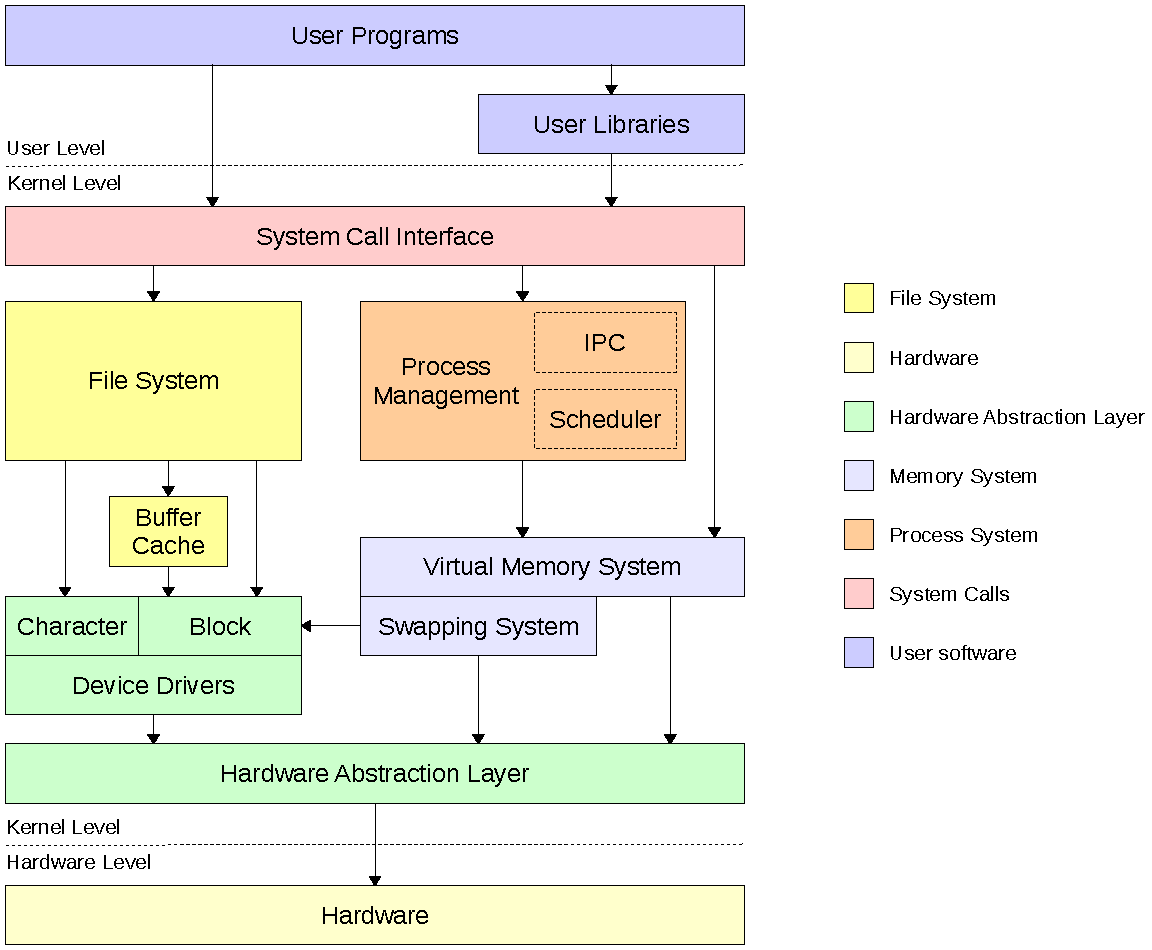
\includegraphics[scale=0.65]{img/nanvix-architecture}
	\caption{Nanvix architecture.}
	\label{figure: nanvix architecture}
\end{figure}

\subsection{System Services}
\label{section: system services}

\subsection{Hardware Requirements}
\label{section: hardware requirements}

\end{document}